\chapter{Benchmarking Tool Implementation}
\label{ch:Framework}
%\section{Benchmarking Framework Development}

It is imperative to establish a standardized pipeline encompassing the entire process, from pre-processing the data to extracting relevant features and validating the algorithm's performance to promote the comparability and reproducibility of brainwave authentication algorithms, \cite{moabb}. By adopting a common pipeline framework, researchers can ensure consistency and facilitate the evaluation of different brainwave authentication algorithms. It also enables the researchers to spend more time on algorithm design and evaluation rather than doing repetitive and error-prone tasks. The common pipeline will be implemented as a wrapper around the scikit-learn pipeline library, known for providing various tools for programming machine-learning models. Moreover, using the scikit-learn library to construct standardized models guarantees credibility, as the pipeline offered by scikit-learn is widely trusted within the machine learning community. Adopting a standardized benchmarking framework will contribute to advancing brainwave authentication techniques, facilitate collaboration, and expedite progress in the field. 

\section{Loading Datasets}
\label{sec:Framework:Loading Datasets}
The datasets, as discussed in section \ref{sec:Solution Approach:Survey Open Datasets: Overview of the selected Datasets}, offer a comprehensive and varied collection of data points, exhibiting notable variations in ERP paradigms, sample size, and subject sessions, are crucial for our study. The wide range of datasets available presents a compelling prospect for conducting comprehensive analysis and exploration. However, the heterogeneous nature of the datasets offers difficulty in their utilization and data management, particularly when performing various analyses and evaluating new algorithms.
To overcome these obstacles and enhance the efficiency of accessing the datasets, a python interface is developed. The purpose of this interface is to optimise and enhance the process of accessing and managing these datasets. The interface utilizes the MNE Python package's capabilities, a comprehensive and versatile software package specifically developed for various tasks such as data preprocessing, source localization, statistical analysis, and functional connectivity estimation among spatially distributed brain regions \cite{MNE_package}. The python interface employs the MNE package to access and arrange public datasets into a hierarchical structure consisting of subjects, sessions, and discrete recordings within each session \cite{moabb}.  The hierarchical structure of data facilitates efficient data management, enhancing the ability to navigate and retrieve specific data as required.
\smallskip

Once the datasets are loaded locally, the raw EEG data are transformed into a standard MNE data format. Standardizing the unprocessed EEG data into raw MNE data is crucial as it is the foundation for all subsequent steps like pre-processing, feature extraction, and evaluation. While converting unprocessed brain data into standardized MNE data, the following actions were followed to ensure consistency across the datasets and to incorporate all pertinent brain samples into the unprocessed MNE data.  
\begin{itemize}
\item EEG data can be quantified in micro voltage or on a voltage scale. The choice of measuring scale is contingent upon the specific EEG devices researchers employ. Upon analyzing our chosen datasets, it was observed that ERPCORE: N400, Mantegna, and COGBCI exhibited congruity in their measurement scale. However, the BrainInvaders15a dataset was originally measured on a micro voltage scale. To ensure consistent data scalability across all four datasets, we rescaled the EEG data of BrainInvaders15a.
    
\item In accordance with the information presented in Section \ref{sec:Solution Approach:Survey Open Datasets: Overview of the selected Datasets}, it has been established that the Mantegna dataset consists of three distinct categories of events, namely congruent, intermediate, and incongruent. According to the research conducted by Mantegna et al., \cite{mantegna2019distinguishing}, it was observed that both intermediate and incongruent stimuli evoke the N400 effect. Based on the observation mentioned earlier, we opted to merge the intermediate and incongruent stimuli into a unified category, denoted as 'incongruent' within the context of our research. This strategy was implemented to bring attention to individual differences in the EEG induced by these stimuli, specifically the N400 ERPs.  

\item Researchers commonly use button press method to record time locked responses to stimuli to guarantee participants focus on EEG activities and the reliability of recorded brain responses. The conventional approach entails utilizing online processing, wherein researchers selectively retain events that elicit accurate responses while disregarding those that indicate a lack of attention. This methodology effectively excludes brain responses that may be random and do not accurately represent ERPs. The same online processing method was observed in the BrainInvaders15a, Mantegna, and ERPCORE: N400 datasets in our study. However, the dataset provided by the COGBCI did not adhere to this particular practice, which necessitated the implementation of offline processing. In this instance, we kept both the congruent and the incongruent time events accompanied by accurate participant feedback, increasing the dataset's utility for ERP research.

%It is seen common practise in EEG experiments to ask the participants to respond to the stimuli by pressing the button. This is done to ensure that the participants are paying attention to the EEG task and that the researchers are recording the correct brain responses. Most of the researchers do online processing where they keep the events where particpants have responded correctly and delete the events where participants was not paying attention and then provide the datasets in the public domain. It does not make sense to include the events where particpants wasn't paying attention, such types of brain responses could be random and does not capture the ERP responses.   
%For our study, we found that researchers of datasets BrainInvaders15a, Mantegna and ERPCORE : N40 have done the  online processing but COGBCI dataset did not. Therefore, we have offline processing on COGBCI where he have kept the congruent and incongruent events for our study where participants has given the correct feedback by pressing the button. 
\end{itemize}
  

%Additionally, as mentioned in section 4.1.2 that dataset mantegna had three kind of events, namely congruent, intermediate and incongruent and it was established in their study \cite{mantegna2019distinguishing} that intermediate and incongruent both produces the N400 effects. As a result, we have merged the intermediate and incongruent stimuli and use them as incongruent stimuli for our study.      

%Unlike other benchmarking frameworks where datasets are usually placed on the local machine and then they are ready every time from the local machine, every time, we tried to try to do benchmarking. For our study, we have devised a more flexible approach to access open datasets.  So, we made a module for dataset in our framework which provides the abstract the open datasets. Basically, any time if some researchers want to see the evaluate the performance of any dataset across different algorithms. As a result, a Python interface utilizing the MNE package \cite{MNE_package}, has been developed for downloading and sorting recorded data into a hierarchy of subjects, sessions, and discrete recordings per session \cite{moabb}. The datasets can be downloaded anytime just by calling the python interface whenever we want to work on those datasets.

%Only the name of the dataset must be mentioned. And the tool will scrap the dataset from the internet, store the data locally and then convert the raw unprocessed data into MNE raw object \cite{MNE_package}. It must be noted that the dataset would be scraped to downloaded from the internet if it is not already available on the local machine. However, if the dataset is already downloaded and stored on the local machine, then the scrapping process will be skipped. Hence, the dataset download is a one-time process. So, by providing the abstract access to the datasets, we have streamlined the access to open datasets. Additionally, EEG datasets are not like conventional datasets where we had one kind of data. Brain datasets differ in terms of format, paradigms, cognitive tasks, number of samples per subject and sessions per subjects and because of that, researchers also spend time, downloading and converting the raw data into a readable format. However, using our framework, the researchers need not to spend time, downloading the datasets and spending writing code to process the data for further analysis. 

\section{Pre-Processing}
\label{sec:Framework:Pre-Processing}
After the datasets have been loaded, it is necessary to establish the pre-processing procedures for EEG data. Various methods exist for cleansing artifacts; however, the procedures must remain consistent to ensure the validity of comparisons between algorithms or datasets \cite{moabb}. 
%As mentioned in section 2.4, The raw EEG data is commonly subject to interference from electrical artifacts. The prevalent sources of such disturbances include electromagnetic interferences generated by nearby electronic devices operating at frequencies of 50 or 60 Hz and muscular artifacts resulting from facial and ocular movements \cite{survey_brain_biometrics}. 
We have adhered to established best practices commonly employed in pre-processing methodologies within brainwave authentication studies \cite{survey_brain_biometrics}. 
The first stage of EEG data cleaning involves the elimination of line noise originating from electronic devices present within the experimental environment during the EEG recording. The application of finite bandpass filtering in the 1 to 50 Hz range is employed for this purpose. The selected range was determined based on the objective of eliminating the 50Hz line noise and filtering out signals originating from flat channels with frequencies below 1 Hz. Figure \ref{fig:PSD strength after band pass filtering} (a) depicts the unprocessed raw signal, which exhibits a significant signal strength at 50Hz due to line noise. On the other hand Figure \ref{fig:PSD strength after band pass filtering} (b) illustrates the consequences of implementing a bandpass filter, revealing a noticeable stabilization in the raw signals after the filtration of the data.  
\begin{figure}
    \centering
    \subfloat[\centering Line noise at 50 Hz due to electrical appliances around the EEG devices]{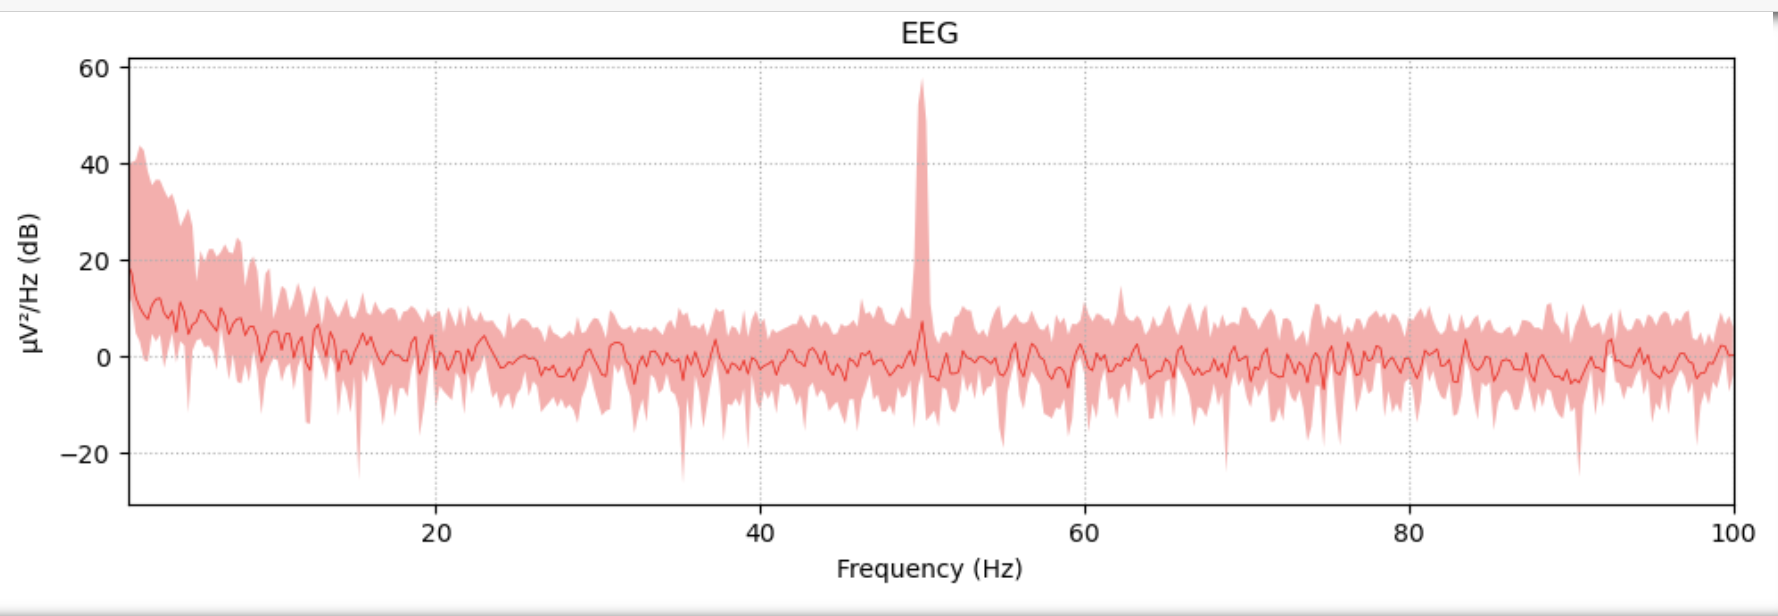
\includegraphics[width=0.75\textwidth]{figures/BrainInvaders15a/raw_psd_plot.png}}
    \\
    \subfloat[\centering Filtered brain signal after applying finite band pass filtering]{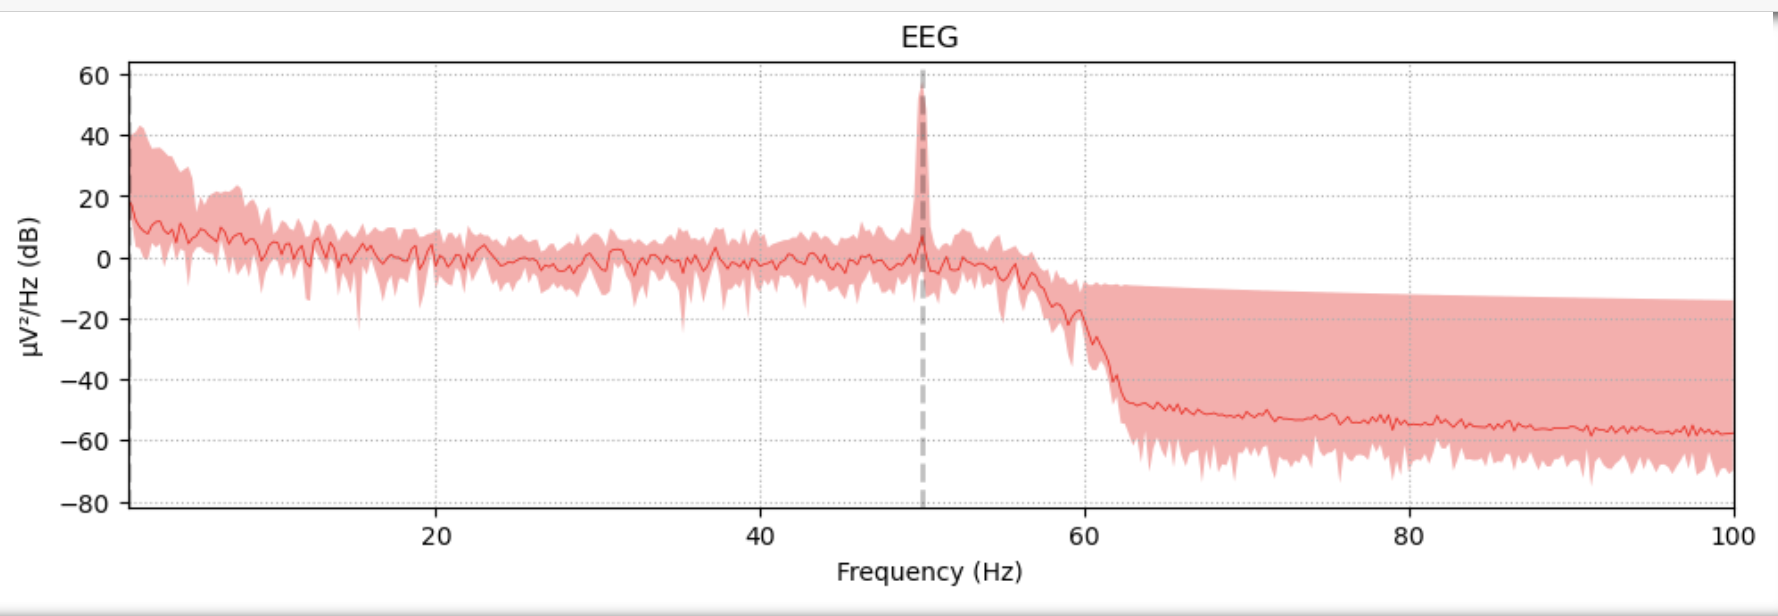
\includegraphics[width=0.75\textwidth]{figures/BrainInvaders15a/raw_filtered_psd.png}}
    \caption{Power Spectral Density of the brain signal before (a) and after (b) applying filtering}
    \label{fig:PSD strength after band pass filtering}
\end{figure}
%Further, the band pass filtering between 1 to 50 Hz  segregate the other artifacts (e.g., electronic signals, eye blinking, muscle contraction, and eye movements) from the signals of interest. 

The subsequent procedure involves the extraction of epochs from the raw signals. The data is temporally aligned to a range spanning from -200 to 800 ms relative to the onset of the stimulus. Baseline correction was applied to each epoch by 
subtracting the mean baseline period, which ranged from -200 to 0 ms. Baseline correction is employed to reduce the drifting effects of DC offsets \cite{fallahi2023brainnet}. Much noise from higher frequencies, such as power lines or very low frequencies from flat channels, is removed during filtering. Nevertheless, the epoch data would still contain certain large artifacts caused by eye or muscle movements that need to be isolated. In practice, it is common to employ thresholds approximately equal to 100$\mu$V or 150$\mu$V in order to eliminate these artifacts effectively \cite{survey_brain_biometrics}. However, this method also results in the loss of a significant amount of valuable EEG data. As illustrated in figure \ref{fig:Peak to peak rejection}, thresholds of 100$\mu$V and 150$\mu$V resulted in the exclusion of over 80$\%$ of the total EEG data for datasets such as BrainInvaders15a and COGBCI. Consequently, we sought to identify an alternative approach that would effectively eliminate the presence of noisy data while minimising the loss of valuable EEG data.
\smallskip

We implemented a more sophisticated approach to eliminate noisy data by utilizing the \textit{Autoreject} \cite{jas2016automated} package. This python package was developed by the original developers of the MNE package, but it has not yet been incorporated into MNE. The Autoreject method addresses the issue of manually determining a threshold by implementing cross-validation on the epochs, allowing for the learning of an optimal rejection threshold specific to each channel. It removes epochs with greater precision and partially repairs them through interpolation techniques. While this method saves a substantial amount of data and corrects noisy trials, we observed that its strategy of performing cross-validation on all user samples could result in data leakage. This prompted us to reevaluate the optimal threshold for rejecting artefacts. We were unable to employ low threshold values, such as 100$\mu$V and 150$\mu$V, nor use Autoreject.
\smallskip

%We also tried an advanced way of removing the bad data by employing \textit{Autorteject} package \cite{jas2016automated}. This python package is developed by the original developers of MNE package but this package is yet to become the part of MNE. Autoreject solves the problem of manual setting of threshold by applying cross-validation on the epochs to to learn a sensor-specific rejection threshold remove trials/epochs with finer precision and/or partially repair them using interpolation. While this approach saves lot of data and also repairs the bad trials, we observed that its approach to perform cross-validation among all the user's samples could lead to data leakage.  
%We also tried an advanced way to drop the noisy samples by using autoreject package \cite{jas2016automated}.  
Consequently, a decision was made to raise the threshold for artifact rejection to 250$\mu$V. A threshold of 250$\mu$V does not represent an extreme threshold for rejecting artifacts, as it falls within a moderate range. The selected value is also based on the consideration that setting a threshold higher than 250$\mu$V would result in the retention of numerous noisy samples in our pre-processed data. Consequently, the subsequent stages, such as classification, would have yielded random predictions due to including random noisy samples. Hence, the implementation of epoch rejection using a peak-to-peak threshold of 250$\mu$V was applied in our study. After performing all the aforementioned pre-processing steps, we averaged the Target(unusual stimuli) and Non-Target(standard stimuli) epochs to check if the ERP signal had been correctly segregated and that the applied pre-processing had successfully minimized other non-task-related brain responses. The visual representation shown in Figure \ref{fig:ERP Graph} depicts the mean evoked potentials seen in the epochs of dataset BrainInvaders15a. The pre-processing steps described above resulted in a total of 4539, 2193, 2097, and 2618 cleaned epochs for the datasets BrainInvaders15a, COG-BCI: Flanker, ERPCORE:N400, and Mantegna, respectively. These epochs are subsequently employed for feature extraction and the classification process. 
\smallskip

%After completing all of the previously indicated pre-processing steps, the epochs are obtained in a clean form. The visual representation shown in Figure \ref{fig:ERP Graph} . These pre-processed are further used to extract features and evaluate various techniques 
%Finally, we obtain the processed epoch signals, which are then used to extract features and evaluate various techniques.
%Artifact rejection has been attempted using threshold values commonly employed, such as 100$\mu$V and 150$\mu$V, as well as higher thresholds of 200$\mu$V and 250$\mu$V. The use of stringent threshold values, such as 100$\mu$V or 150$\mu$V, for artifact rejection is a common approach to remove noisy signals through peak-to-peak rejection. Consequently, a decision was made to raise the threshold for artifact rejection to 200$\mu$V.
\begin{figure*}
    \centering
    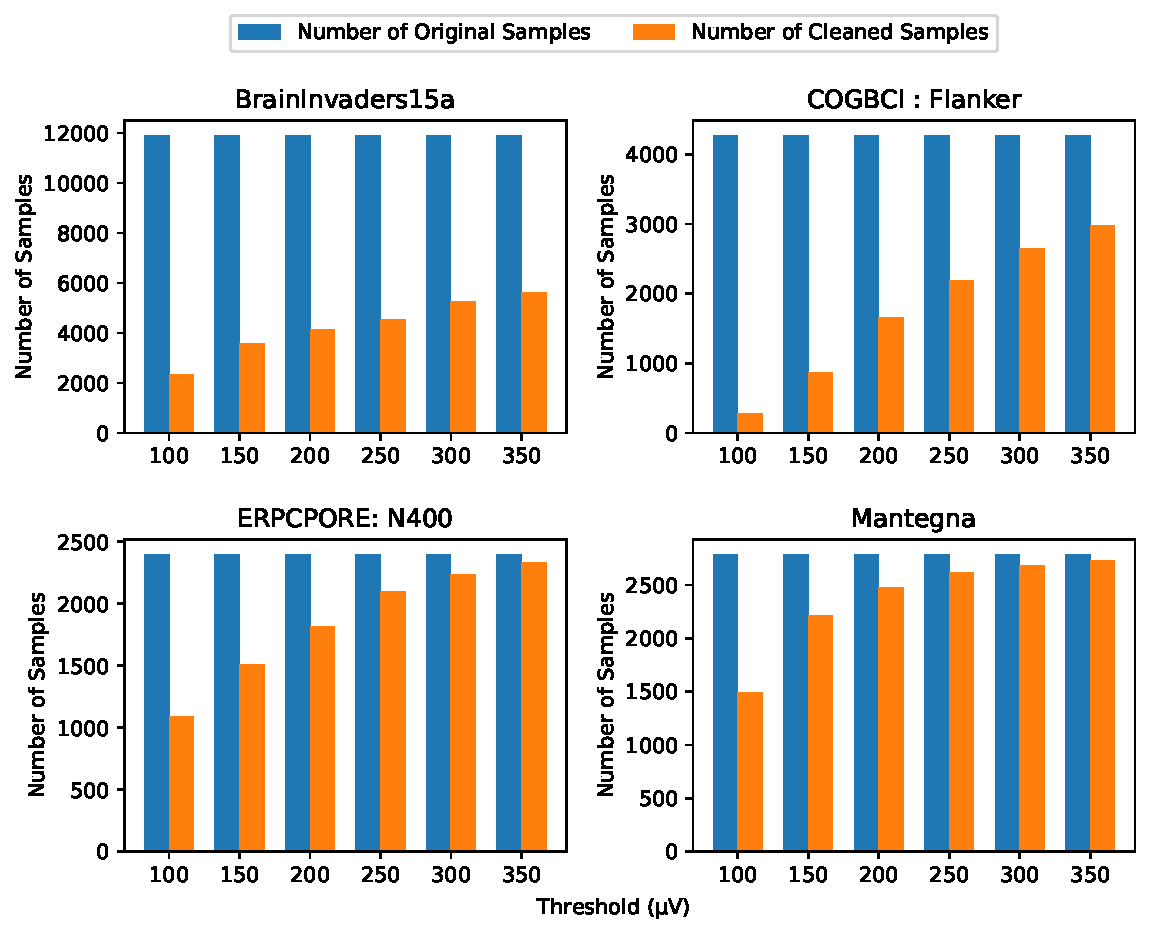
\includegraphics[width=0.75\textwidth, height=0.8\textheight, keepaspectratio]{figures/peak_to_peak_threshold.pdf}  
    \caption{Actual number of epochs versus the number of cleaned epochs after conducting epoch rejection with various thresholds. X-axis depicts the sample count whereas y-shows the threshold values in $\mu$V}
    \label{fig:Peak to peak rejection}
\end{figure*}

\begin{figure*}
    %
    \centering
     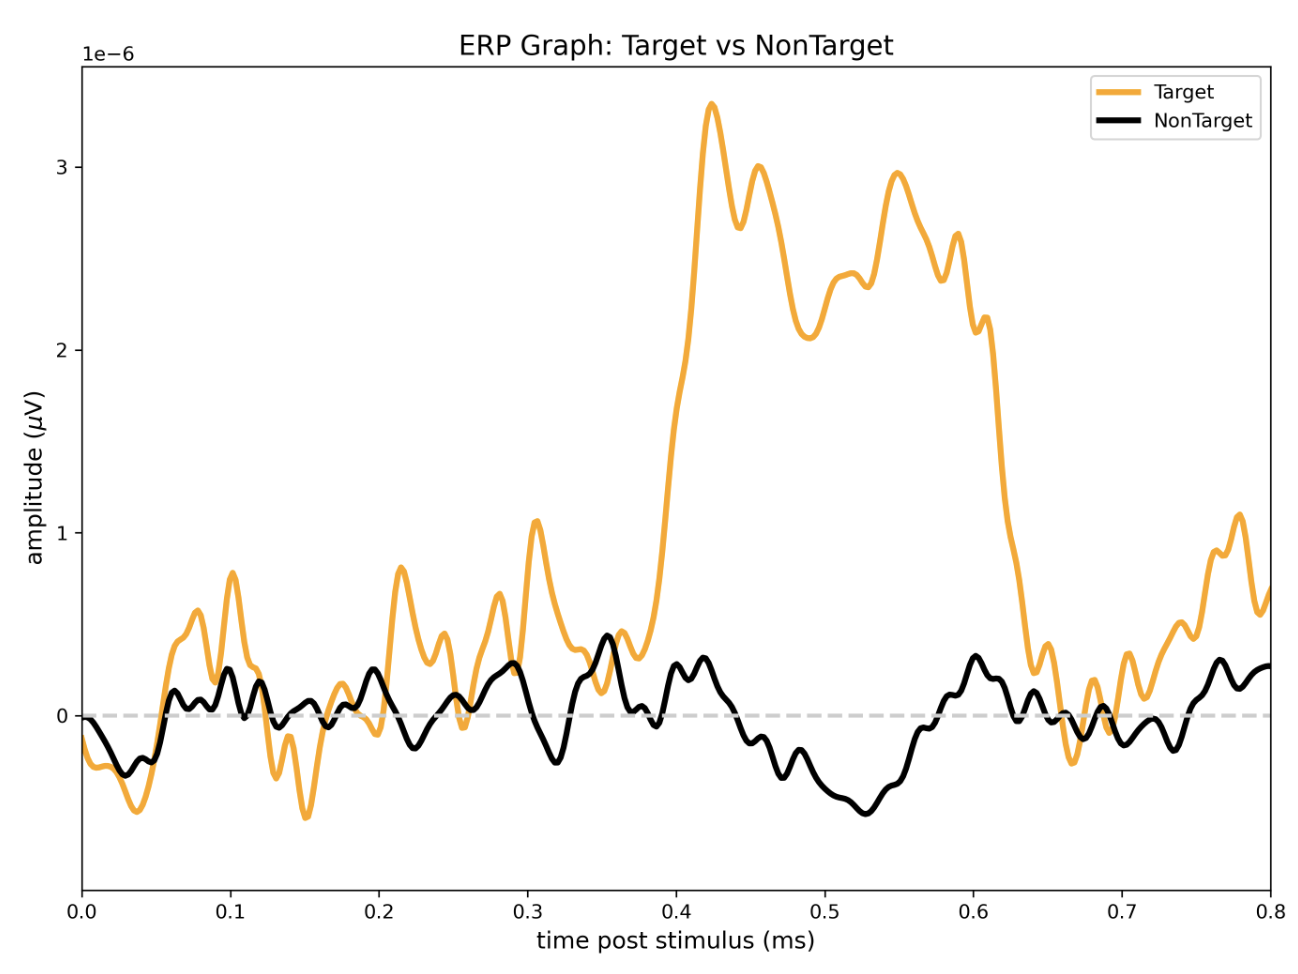
\includegraphics[width=0.75\textwidth]{figures/BrainInvaders15a/erp_graph_1.png}  
    %
    
    %\caption{SMC Learning Algorithm}
    \caption{The Averaged Evoked Potentials exhibit an increase in amplitude ranging from 250 to 400 milliseconds, which can be attributed to the implementation of the oddball paradigm}
    \label{fig:ERP Graph}

 \end{figure*}
%After completing all of the previously indicated pre-processing steps, the brain samples are obtained in a clean form. The visual representation shown in Figure 4.6 depicts the mean evoked potentials seen in the brain sample of dataset BrainInvaders15a after all necessary cleaning operations.
  
%Following the completion of all of the previously indicated pre-processing steps, the brain samples are obtained in a clean form. Our standardised cleaning process yielded cleaned epochs that may be averaged for both target and non-target events. The visual representation shown in Figure 4.6 clearly depicts the mean evoked potentials seen in the brain sample of dataset BrainInvaders15a after all necessary cleaning operations. Finally, we obtain the processed epoch signals, which are then used to extract features and evaluate various techniques.  

%A lot of noise from higher frequencies such as power lines or, very low frequencies coming from the flat channels, gets removed during the filtering step. However, the epoch data would still be having some artifacts which are required to isolate. Therefore, automatic epoch rejection has to be applied based on the peak-to-peak amplitude of electrodes. 

%Finally, the cleaned epoch signals will be utilized for feature extraction and evaluation of different algorithms.  


%Once datasets are loaded, the
%pre-processing steps of EEG data need to be defined. There are multiple ways to clean the artifacts but the processes need to be the same for comparisons between algorithms or datasets to be valid \cite{moabb}. We will some of the best steps taken us to remove the artifacts. As already is discussed in section 2.4, The raw EEG data is generally very noisy due to various artifacts such as eye blinks, muscle movements, line noise from nearby electronics devices. WE choose to follow some of the best practices followed for pre-processing in brainwave authentication studies. The first step in EEG data cleaning is to remove the line noise from the electronics devices, present in the room during the EEG experiment. This is done by applying the band pass filtering between 1 to 50. We choose this range to remove the 50 Hz line noise as well remove the signals from flat channels with less than 1 Hz frequency. In Figure 4.5 left image illustrates the unprocessed raw signal where it is huge signal strength at 50 Hz due to line noise. And in the same image,  right side image depicts aftermath of applying band pass filtering and we can see there is some stabilization in the raw signals once the data was filtered.  

\section{\large Feature-Extraction}
\label{sec:Framework:Feature-Extraction}
After pre-processing the EEG data, the next step is to acquire discriminant features that represent and encode a user's mental activity using the clean EEG signal \cite{survey_brain_biometrics}. We surveyed many studies presented for brainwave authentication. We found
that the Autoregressive (AR) model and Power spectral Density (PSD) are some of the most widely used methods for extracting features in time and frequency domains \cite{arias2023performance, arias2021inexpensive}. Further, AR's potential to reveal particular inherent characteristics of the EEG signal within a single channel and PSD's ability to extract and distinguish the dominant frequency components \cite{survey_brain_biometrics} make them a promising candidate for our study to extract subject-specific information from the EEG data. Our research's feature extraction procedure, which uses the above mentioned techniques, is outlined below.  
\begin{itemize}
\item \textbf{\large AR Coefficients}: 
The AR model is fitted using pre-processed epochs, time series data lasting for 1 second \cite{arias2023performance}. The coefficients obtained from this procedure are subsequently considered as features. The estimation of AR coefficients can be accomplished by utilizing the Yule-Walker method. The Yule-Walker method is a computational approach that employs a pth-order AR model to analyze a signal subjected to windowing. This is accomplished by minimizing the least square error of forward prediction and directly solving for the AR parameters \cite{pardey1996review}.
%Each pre-processed epoch, a time series lasting for 1 second, is utilized to fit an AR model \cite{arias2023performance}. The resulting coefficients from this process are then regarded as features. AR coefficients can be calculated by using the Yule-Walker method. The Yule-Walker method is a technique that uses a pth-order AR model to analyze a windowed input signal. It achieves this by minimizing the least square error of forward prediction and directly solving for the AR parameters.
\smallskip
Identifying the optimal order for AR modeling is an intricate task since high orders increase the computational cost and very low order does not represent the signal properly \cite{zhang2017classification}. As a result, We extracted AR features in various orders, such as 1, 2, 3, 4, 5, 6, 7, 8, 9, and 10. However, the most optimum order appears to be 6, and we have set the default order to 6 in our framework. It is important to acknowledge that the AR coefficients are computed individually for each channel within the signal. Therefore, the total number of AR coefficients calculated is proportional to the number of channels utilized for feature extraction. For instance, in the scenario where brain data is analyzed through the utilization of 32 channels, and all of these channels are employed for the feature extraction process, it can be observed that the application of a 6th-order AR model will yield a total of 196 features (32 channels multiplied by an order of 6).  

\item \textbf{\large PSD}: The PSD of each epoch is computed across different frequency bands, namely low (1-10 Hz), alpha (10-13 Hz), beta (13-30 Hz), and gamma (30-50 Hz), utilizing the Welchs periodogram algorithm \cite{arias2023performance}. Welch's periodogram is used to compute the Discrete Fourier Transform (DFT) results \cite{survey_brain_biometrics}. In our study, first the power spectral density (PSD) for each frequency point in 1-second epoch is calculated. Furthermore, in calculating PSD using Welch's algorithms, we utilized four-time windows of equal size on a 1-second ERP epoch, with 50$\%$ overlap between each window. Including the time window factor was necessary to separate the genuine frequency modulation of the EEG caused by attention from any artifacts that the attentional modulation of ERPs may have induced \cite{comez1998frequency}. We then computed the average PSD within the specified frequency ranges.  This allowed us to determine the average power spectrum of the low, alpha, beta, and gamma frequency bands. Similar to the AR features, the PS features are likewise computed for each channel.    

%The Power Spectrum (PS) of each epoch is calculated in various frequency bands such as low (1-10 Hz), alpha (10-13 Hz), beta (13-30 Hz), and gamma (30-50Hz) using the Welchs periodogram algorithm \cite{arias2023performance}. The welch's periodogram is employed to calculate the Discrete Fourier Transform (DFT) results. Additionally, while calculating PSD using welch's algorithms, we employed 4 equal sized time windows on 1-second ERP epoch, with 50$\%$ overlap between each periodogram. 

\end{itemize}
\section{Classification}
\label{sec:Framework:Classification}

Most brainwave authentication techniques fall under the categories of similarity-based or supervised learning-based recognition systems \cite{survey_brain_biometrics}. In our study, we have employed both learning methods for authentication. Additionally, classification is performed under two evaluation strategies: within-session and cross-session. We undertake a comparative analysis and examination of the suitability of two evaluation schemes and authentication methodologies for various classifiers within two threat case scenarios. The subsequent sections delineate the methods for conducting authentication within the context of similarity or supervised learning techniques.
%\subsubsection{Classifiers}:
\subsection{\large Supervised based Learning Classification}
\label{sec:Framework:Classification:Supervised based Learning Classification}
Authentication is performed by comparing the user’s recorded samples with the user’s enrolled samples, usually stored during the registration phase, to classify whether the recorded samples match. The fundamental concept entails acquiring knowledge through the utilization of a one-vs-all classification methodology employing a binary classification system with two distinct classes. Consequently, a classifier is trained for each subject to be incorporated into the system. Accordingly, a singular classifier is tasked with recognizing an individual issue \cite{arias2023performance}. Traditional classifiers like LDA, SVM, RF, GNB, LR, and KNN are utilized in this study to classify the features we calculated in the feature extraction process. The classification will be performed under the within-session and cross-session evaluation schemes detailed below.

\subsubsection{Within-Session Evaluation}
Under the within-session evaluation, the training and testing of the features are done utilizing the recorded data from a single session. To avoid overfitting and increasing the reliability of our authentication system, we used RepeatedStratifiedKFold (k=4) to split the single session data into training and testing. Stratified cross-validation was chosen because it ensures that the features from both classes are represented in the train and test data during each fold. Users with less than four samples were eliminated from the datasets to ensure adequate samples for both training and testing \cite{arias2023performance}. The total number of repetitions conducted was 10, and the results of the evaluation metrics are obtained all folds, and runs are averaged and reported.
Additionally, we employed feature scaling to prevent overfitting by fitting the StandardScaler \footnote{\url{https://scikit-learn.org/stable/modules/generated/sklearn.preprocessing.StandardScaler.html/}} on the training set and applying it to both the train and test sets in every iteration. In the dataset, such as COGBCI, which has multiple sessions across subjects, the evaluation has been performed across each session. Then the results from the three sessions have been averaged. 
\smallskip

\textit{Threat Case Scenarios}: The implementation and evaluation of an authentication system across individual sessions are conducted in the context of two attack scenarios: Close-set scenario is a standard one vs all approach described earlier in this chapter. Under this approach,  
we trained unique classifiers for each user by marking all of their samples as "authenticated" and all of the samples from all other users as "rejected" \cite{arias2023performance}. The close-set approach has been extensively utilized in numerous studies. The current process lacks real-world applicability as it operates under the assumption that attackers are already part of the system, making it simpler for the model to distinguish genuine users. However, this is only sometimes the case, as the attacker could be an unknown user attempting to imitate a legitimate user. Hence, assessing the authentication system's efficacy in an open-set scenario is imperative. However, implementing an open set is more challenging due to the requirement of training the classifier with known users (enrolled users) and evaluating it with unknown users (attackers who are completely known to the system). We looked, and unfortunately, no cross-validation technique exists that meets all of our requirements for training and testing in an open-set environment. Thus, we adopted a tailored cross-validation approach to test the robustness of our authentication system in an open-set scenario. 

We separated dataset samples into 'authenticated' and 'attackers' groups to implement an open-set scenario. A GroupKFold strategy with a value of K=4 was utilized, wherein 'attackers' SubjectIDs were employed. The data were divided into training and testing, with 75$\%$ attackers allocated to training and the remaining 25$\%$ assigned to testing in each cross-validation. Each cross-validation iteration constructed a modified training set by randomly selecting 75$\%$ of the 'authenticated' samples and the majority (75$\%$) of the 'attackers' samples. The testing set, on the other hand, comprised the remaining 'authenticated' and 'attackers' samples. This GroupKfold method ensured a non-overlapping distribution of 'attackers' participants between training and testing, improving our system's practical validity in real-world settings. For example, ERPCORE: N400 dataset contains 40 individuals. In this scenario, the epochs of a user are assigned authenticated labels, with 29 being rejected and 9 identified as unknown attackers per model \cite{arias2023performance}.  9 unknown attackers were absent in the training set. The model is trained and tested using a train-test split of 75$\%$ and 25$\%$, respectively. 


%our model incorporates one 'authenticated' user label and 29 'attacker' labels for training in each cross-validation iteration. In the testing phase, the dataset consists of one label assigned to an 'authenticated' user and nine labels assigned to 'unknown attackers,' which were absent in the training set. Similar to close-set, features were scaled using standardscaler before fitting into the classification algorithm. 

%For example dataset ERPCORE: N400 has 40 subjects. In this case, the model contains one authenticated user labels, 29 attackers labels in training and one authenticated user labels and 9 unknown attacker labels. 



%While close-set approach had been widely adopted in many studies. It does not provide the real word implementation since this approach assumes that the attackers are part of the system and therefore, easy for the model to identify the genuine user. However, this not always the case as the attacker can be an unknown user, trying to impersonate a genuine user. Therefore, it is essential to evaluate the performance the authentication system under the open-set scenario. While close-set is rather easy to implement using stratified cross-validation, open-set is rather tricky to implement because under this approach, the classifier needs to be trained with known users i.e., enrolled users and then evaluated with unknown users i.e. attackers completely unknown to the system. We checked and there is no existing cross-validation method which can fulfil our training and testing under open-set scenario. As a result, implemented a modified cross-validation method to evaluate our authentication system under open-set scenario. 


\subsubsection{Cross-Session Evaluation}
The collection of multi-session EEG recordings poses challenges as it becomes more difficult to ensure that all participants can replicate the experiment accurately after a designated period \cite{huang2022m3cv}. It is also the underlying cause of the significant scarcity of datasets. In our study, we have s single multi-session dataset out of all the open datasets, i.e., COGBCI, which contains 3 recorded sessions at an interval of 7 days. Each session consisted of a full duration of 10 minutes. As a result, we performed the cross-session evaluation on this dataset. Under the cross-session evaluation strategy, two sessions containing 20 minutes of EEG recording data are used for enrollment or training the classifier.
In contrast, the remaining session data is employed for testing or authentication. This approach ensures the substantial data of model training, ensuring the reliability of the resultant classifier. The performance of the model is assessed in a distinct and independent session. A cross-validation strategy is employed to avoid potential bias in session allocation. We used LeaveOneGroupOut \footnote{\url{https://scikit-learn.org/stable/modules/generated/sklearn.model_selection.LeaveOneGroupOut.html}} cross-validation method to group the sessions into training and testing set. The issue of potential overfitting was addressed by applying feature scaling to the training and testing set. Jayaram and Barachant \cite{moabb} implemented a comparable cross-session evaluation approach in their development of MOABB (Mother of all BCI Benchmark), a benchmarking framework evaluating the performance of different BCI algorithms on open datasets. Additionally, we excluded users who did not have at least three sessions of data to ensure an adequate number of samples in both the training and testing sets. Just like within-session evaluation, classification in cross-session is also conducted using both threat case scenarios.
\smallskip

\textit{Threat Case Scenarios}: 
This evaluation scheme includes both closed-set and open-set scenarios. A single classifier is trained to recognize each user in a close-set method. To meet this criterion, samples from a specific user across all three sessions are labeled "authenticated," while samples from all other users are labeled "rejected."  The training set consists of data from two out of three sessions and includes authenticated and adversary samples. During testing, the remaining session data is utilized.
The close-set method is comparable to the one described for within-session evaluation, with the exception that the model is evaluated using data from multiple sessions and therefore, more realistic. However, our study goes beyond the close-set scenario and investigates the system's efficacy when exposed to unknown attackers during authentication in a cross-session environment. 
\smallskip

The open-set scenario follows the same method of LeaveOneGroupOut cross-validation for grouping session data into training and testing sets. But to accommodate the open-set strategy, we modify the composition of the attackers within these sets. In each round of the cross-validation, a random selection is made, based on the SubjectIDs, to include 75$\%$ of the attackers in the training set. The training process excludes the remaining 25$\%$ of attackers. In contrast, the testing set comprises solely the attackers that were omitted during the training phase while excluding the attackers on which the model was trained. By employing this methodology, we effectively establish a scenario wherein the model is evaluated using attackers entirely unknown to the system in a cross-session environment. 

%But to facilitate this strategy for open-set, during eac round of cross-validation, we randomly selected 75$\%$ attackers based on SubjectID's for training the model and remove the remaining attackers from the training set. We did the extract opposite for testing set where we retain the attackers which were removed while training and excluded the attackers from the testing set on which the model was trained. By doing this, we implemented the open-set scenario where the model is evalauted on attackers completely unknwon to the system.  

%It must be noted that single classifier is responsible for recognising the individual user. As a result, we labelled the users into 'authenticated' and 'rejected' in each session before passing the data for cross-validation. 


%\subsubsection{}
%\textit{Close-Set Scenario}
%\smallskip

% \textit{Open-Set Scenario}
% \smallskip

% \subsubsection{\large Cross-Session Evaluation}
\subsection{Similarity Based Learning}
\label{sec:Framework:Classification:Similarity Based Learning}
Unlike Supervised learning methods, which entail training a model with other users for decision-making \cite{fallahi2023brainnet}, similarity-based techniques identify a person based on the similarity between the brain signals acquired during the enrollment phase and those presented during the verification phase. The similarity between the enrolled and tested samples is calculated using metrics like Euclidean or cosine distance. Siamese Neural Networks (SNN) is a highly effective deep learning (DL) method for implementing similarity metrics for brainwave authentication, employed already in studies such as \cite{fallahi2023brainnet, seha2020eeg, maiorana2019eeg}. This type of learning allows for accurate predictions after training the network with only a few samples \cite{facenet}, overcoming a typical drawback of employing DL approaches for brainwave authentication. It also avoids the usual shortcoming of supervised learning algorithms—retraining—while adding new users to the system, as discussed in subsection \ref{sec: Introduction:Solution Overview}. 
\smallskip

In the context of classification, supervised algorithms frequently require extracting discriminant features from raw epochs to enhance the classification process. In contrast, the SNN method adopts a distinct strategy by circumventing the conventional feature extraction procedure. Instead, it generates feature embeddings directly from the time series data of epochs using the CNN method. The epochs are structured in a two-dimensional array, where the rows correspond to channel indices, and the columns represent discrete-time measurements. SNN can be trained using various loss functions such as Contrastive loss function and Triplet loss \cite{ghojogh2020fisher}. Among these, the \textit{triplet loss} approach is particularly well-suited for biometric recognition \cite{fallahi2023brainnet}. As a result, our study utilizes SNN with three CNN branches, which are trained using a triplet loss function. As explained by Schroff \textit{et al.} \cite{facenet} in their study, learning using the triplet loss function involves the provision of three distinct types of inputs, namely an anchor, a positive sample (which shares the same identity as the anchor), and a negative sample (which possesses a different identity than the anchor). Following the completion of this procedure, the embeddings of individuals of the same identity will exhibit minimal distances, while those corresponding to distinct individuals will exhibit significant distances. As a result, once the embeddings are generated, a similarity metric (often Euclidean distance) can be used to verify or identify them. Figure \ref{fig:Triplet Loss} illustrates the learning procedure in SNN using triplet loss function. 
\begin{figure*}
    %
    \centering
     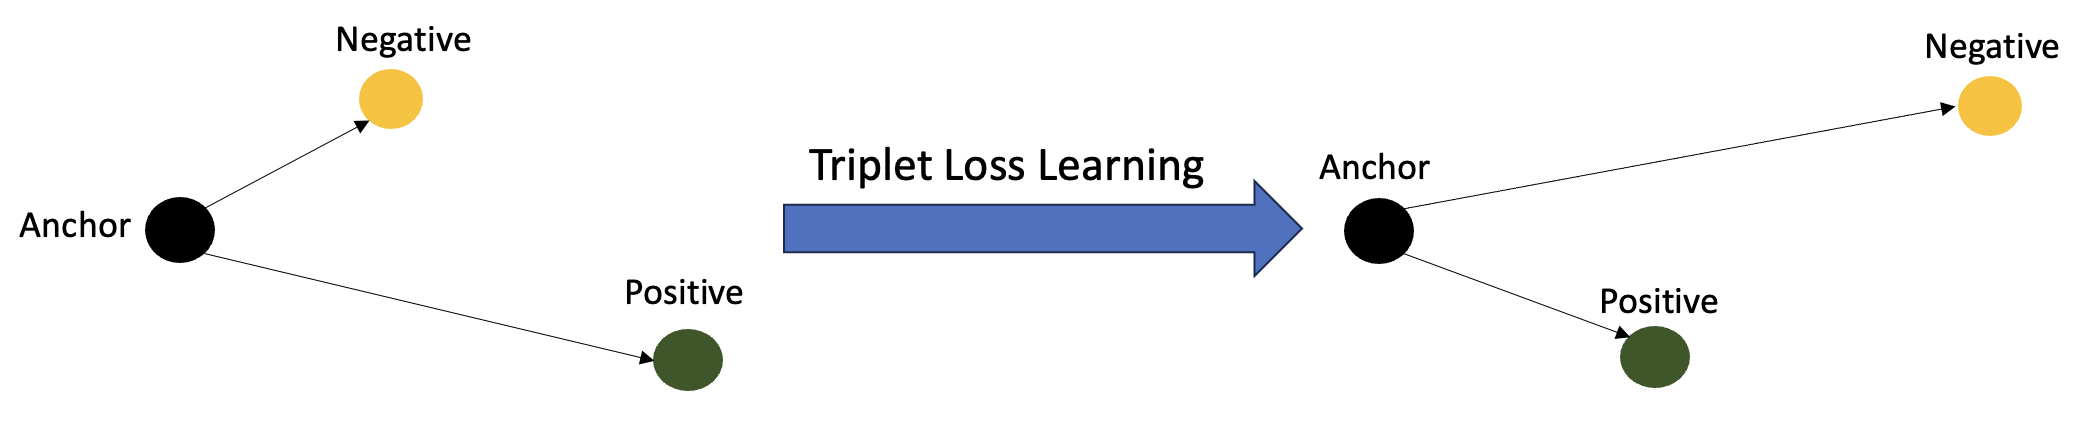
\includegraphics[width=\textwidth]{figures/Siamese/Triplet_loss_updated.png}  
    %
    
    %\caption{SMC Learning Algorithm}
    \caption{Triplet loss function minimizing the euclidean distance between the anchor and positive embeddings while simultaneously maximizing the distance between the embeddings of two different individuals, specifically the anchor and negative embeddings}
    \label{fig:Triplet Loss}
\end{figure*}

The Siamese architecture proposed by Fallahi et al. \cite{fallahi2023brainnet} was implemented in our study. Therefore, a CNN consisting of five convolution layers was utilized to develop the system. After each convolutional layer, an average pooling layer was applied to reduce the input vectors' dimensionality while preserving each brainwave's unique characteristics. Further, the FaceNet study \cite{facenet} demonstrated that minimizing triplet loss through the online mining of semi-hard triplets is the most effective method for quick convergence; consequently, this method of triplet selection was also utilized in our study. Furthermore, user authentication is performed using both within-session and cross-session evaluation strategies outlined below.  

\subsubsection{Within-Session Evaluation}
The within-session evaluation in SNN is designed to work well in both the seen attackers (close-set) and unseen attackers (open-set) scenarios. Both scenarios are implemented in a similar methodology, except the first involves comparing the identification sample with all the enrollment samples during testing. In contrast, in the open-set method, the subject's sample being tested is compared to an enrollment database that does not include the subject's specific brain sample \cite{fallahi2023brainnet}. The comparison is conducted through the computation of Euclidean distance. Below is a short overview of the evaluation strategy for both threat case cases.
\smallskip

\textit{Threat Case Scenarios}: In close-set, the user's samples were divided into training and testing sets using stratified cross-validation with k=4. As a result, we omitted users from the datasets with less than four samples. The SNN model is trained on all the users of the dataset. For example, if the dataset has EEG data of 40 subjects, all 40 subjects get enrolled during the training process. Training and testing data is scaled using the standard scaler normalization method. The model learns to generate the brain embeddings, and during verification, the brain embeddings of each user are compared against the enrollment data of all subjects. 
\smallskip

Implementing the open-set approach involves utilizing the GroupKFold cross-validation strategy, with a value of k set to 4. During each round of cross-validation, the grouping is done based on SubjectID, resulting in a non-overlapping training set consisting of 30 subjects and a testing set of 10 users. The process of evaluating open-set scenarios involves the comparison of each subject's brain sample with the samples contained within the testing set. This approach tests the model's recognition capability against unseen attackers.
\smallskip

\subsubsection{Cross-Session Evaluation}
The methodology utilized for implementing cross-session evaluation in Siamese Neural Networks (SNN) is comparable to the approach employed for the cross-session assessment in supervised learning-based classification tasks. Therefore, LeaveOneGroupOut cross-validation was employed for grouping the sessions into training and testing set in each round of cross-validation.

\textit{Threat Case Scenarios}: A close-set scenario is attained by employing the LeaveOneGroupOut cross-validation technique we discussed previously. In a close set, samples from each subject's independent session are compared to their respective enrollment records. In this instance, the enrollment database comprises the brain samples of all subjects collected during the two sessions. In the open-set scenario, the sessions data is partitioned into training and testing sets using the LeaveOneGroupOut method, where subjects from the enrollment database that are being verified are excluded. The enrollment database in this case has two sessions of data, and the evaluation is based on the remaining session data.  
%In open-set, we divide the sessions data into training and testing using the same LeaveOneGroupOut method but removed subjects from the enrollment database that are being verified. The enrollment database here contains 2 sessions data and evaluation is on the remaining session data.  

%Supervised algorithms ng using the saoften necessitate to extract discriminant features from the raw epochs for the purpose of classification to facilitate classification. However, SNN takes a different approach by bypassing the feature extraction process and instead generates feature embeddings from the time series data of epochs, by utilizing three CNN branches. The branches undergo training using a triplet loss function. 
%SNN skips the feature extraction process, instead it produces feature embeddings by utilizing three CNN branches. These branches are trained with a triplet loss function. 

\subsection{Automated Benchmarking}
The benchmarking framework is developed with a primary focus on ensuring user-friendliness. Our objective was to enable anyone to effectively utilize this framework, even without a comprehensive understanding of the complex technical intricacies underlying the Python programming language. Consequently, a user-friendly benchmarking script was developed, efficiently analyzing a configuration file written in a clear and concise YAML manner. This configuration file is a control panel for defining various parameters and settings. It automates all the complex tasks involved in data extraction, pre-processing, feature extraction, and classification, as illustrated in Figure \ref{fig:Benchmarking suite}. This streamlined approach eliminates the need for users to delve into intricate programming complexities. Appendix \ref{chapter: Appendix} showcases illustrative examples of such configuration files, underscoring the simplicity and accessibility of our framework's implementation.
\smallskip

Examples of configuration files featuring benchmarking pipelines tailored for within-session and cross-session evaluations on a single dataset are showcased in sections \ref{sec:Appendix:Within-Session} and \ref{sec:Appendix:Cross-Session}, respectively. The examples mentioned above effectively illustrate the flexibility and versatility of our methodology. These examples show that the pipelines can be optimized using default dataset values. Furthermore, they can be seamlessly configured to accommodate various parameter variations, spanning dataset specifics, pre-processing techniques, and algorithm selections. We will explain the significance of each parameter applied on the datasets such as \textit{subjects, interval, epochs rejection} in chapter \ref{sec:Evaluation:Results}. In Chapter \ref{sec:Evaluation:Results}, we will delve into an in-depth exploration of the significance underlying each parameter employed on the dataset, including \textit{subjects, interval,} and \textit{epochs rejection}. This comprehensive analysis will shed light on the crucial role these parameters play in shaping the outcomes of our study.
%This demonstrates our benchmarking platform's adaptability and usefulness for researchers looking for customized experiments. 

%The examples of configuration files, having benchmarking pipelines for within-session and cross-session evaluated on single dataset are depcited in \ref{sec:Appendix:Within-Session} and \ref{sec:Appendix:Cross-Session} respectively. As shown in the examples, the pipelines can be degenerated for default parameters of the dataset and they can also be utilized with different parameters of the dataset, pre-processing and algorithms. 

%We developed our benchmarking framework as user-friendly as possible. We wanted that the people can use this framework without having to understand all the technical aspects of the python programming implemented for this framework. Therefore, we created a benchmarking script which will parse the config file written in a very simple maner in .yaml extension and performs all the data extraction, pre-processing, feature extraction and classification steps explained in Figure \ref{fig:Benchmarking suite} automatically. Examples of the configuration files are showin in appendix \ref{chapter: Appendix}. 




